

{\setbeamercolor{background canvas}{bg=black}
	\begin{frame}[plain]
	\vfill
	\begin{columns}
		\column{.5\textwidth}
		\color{tumwhite}
		
		\Huge
		\visible<2->{\color{tumgray} Self-}{\color{white}Attention} \visible<2->{in \\ Deep Learning}
		
		\column{.5\textwidth}
		
		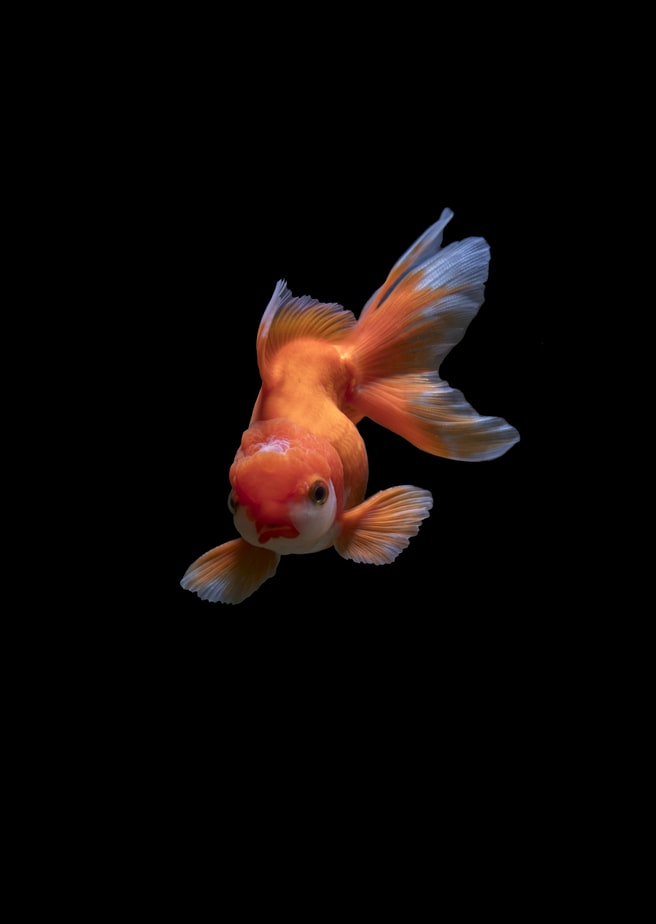
\includegraphics[width=6cm]{images/goldfish_zhengtaoTang}
	\end{columns}
	\begin{center}
		\Huge\color{tumwhite}
		\vfill\raggedleft
		{\small \color{tumgray} Photo by zhengtao tang on Unsplash}
		
	\end{center}
	\vfill
\end{frame}
}

\begin{frame}
	\frametitle{Attention}
	
	\begin{columns}
		\column{.5\textwidth}
		
%		
%		
%		\attention
%		
%		\attnv
		
		\begin{tikzpicture}[node distance=.2em]
		\node[label={below:$\V{\alpha}^T$}, draw=attentioncolor, rounded corners](alpha){\attention};
		\node[right=of alpha](out){\attnout};
		\node[above=of out, label={above:${\only<1,2>{\V{v}}\only<3>{\M{V}}}$}, draw=valuecolor, rounded corners]{\attnv};
		\visible<2->{
		\node[above=of alpha, label={above:$\M{K}$}, draw=keycolor, rounded corners]{\attnkey};
		\node[left=of alpha, label={below:${\only<1,2>{\V{q}}\only<3>{\M{Q}}}^T$}, draw=querycolor, rounded corners]{\attnquery};
		}
		\end{tikzpicture}
		
		%	\begin{equation*}
		%		\text{Attention}(Q,K,V) = 
		%		\begin{tikzpicture}
		%		\node(alpha){$\underbrace{\attention}_\alpha$};
		%		\node[right=of alpha](out){};
		%		\node[above=of out]{\attnv};
		%		\end{tikzpicture}
		%		 
		%	\end{equation*}
		
		
		\column{.5\textwidth}
		
		\begin{tikzpicture}[yscale=3]
			
			\visible<3>{
				\node[draw=valuecolor, circle, fill=valuecolor, fill opacity=.2, text opacity=1, font=\small, inner sep=.2em](d) at (1,.35){};
				\node[draw=valuecolor, circle, fill=valuecolor, fill opacity=.1, text opacity=1, font=\small, inner sep=.2em](e) at (2,.05){};
				\node[draw=valuecolor, circle, fill=valuecolor, fill opacity=.3, text opacity=1, font=\small, inner sep=.2em](f) at (3,.42){};
				\node[draw=valuecolor, circle, fill=valuecolor, fill opacity=.4, text opacity=1, font=\small, inner sep=.2em](g) at (4,.25){};
				\draw (d) -- (e) -- (f) -- (g);
			}
			
			\node[draw=valuecolor, circle, fill=valuecolor, fill opacity=.2, text opacity=1, font=\small, inner sep=.2em](a) at (1,.3){};
			\node[draw=valuecolor, circle, fill=valuecolor, fill opacity=.1, text opacity=1, font=\small, inner sep=.2em](b) at (2,.1){};
			\node[draw=valuecolor, circle, fill=valuecolor, fill opacity=.3, text opacity=1, font=\small, inner sep=.2em](c) at (3,.3){};
			\node[draw=valuecolor, circle, fill=valuecolor, fill opacity=.4, text opacity=1, font=\small, inner sep=.2em](d) at (4,.4){};
			
			\draw (a) -- (b) -- (c) -- (d);
			
			\foreach \t in {1,2,3,4} {
				\draw[tumgray] (\t,0) -- (\t,-.05) node[at end, below, text=tumgray] {$t_\t$};
			}
			
			%\draw[-stealth] (0,0) -- (0,.5);
			\draw[-stealth, tumgray] (.5,0) -- (4.5,0);
			
			\only<1,2>{
			\node[draw=tumblack, circle, fill=attentionoutcolor, text=white, fill opacity=1, text opacity=1, font=\small, inner sep=.2em, label={right:$\sum_{t=0}^{T} \alpha_t v_t = \V{\alpha}^T \V{v}$}](out) at (2.5,-.5) {};
			}
			\only<3>{
			\node[draw=white, circle, fill=attentionoutcolor, text=white, fill opacity=1, text opacity=1, font=\small, inner sep=.2em](outba) at (1.05,-.48) {};
			\node[draw=white, circle, fill=attentionoutcolor, text=white, fill opacity=1, text opacity=1, font=\small, inner sep=.2em](outbb) at (2.05,-.48) {};
			\node[draw=white, circle, fill=attentionoutcolor, text=white, fill opacity=1, text opacity=1, font=\small, inner sep=.2em](outbc) at (3.05,-.48) {};
			\node[draw=white, circle, fill=attentionoutcolor, text=white, fill opacity=1, text opacity=1, font=\small, inner sep=.2em](outbd) at (4.05,-.48) {};
				
			\node[draw=white, circle, fill=attentionoutcolor, text=white, fill opacity=1, text opacity=1, font=\small, inner sep=.2em](outa) at (1,-.5) {};
			\node[draw=white, circle, fill=attentionoutcolor, text=white, fill opacity=1, text opacity=1, font=\small, inner sep=.2em](out) at (2,-.5) {};
			\node[draw=white, circle, fill=attentionoutcolor, text=white, fill opacity=1, text opacity=1, font=\small, inner sep=.2em](outa) at (3,-.5) {};
			\node[draw=white, circle, fill=attentionoutcolor, text=white, fill opacity=1, text opacity=1, font=\small, inner sep=.2em](outa) at (4,-.5) {};

			}
		
			\node at (2.5, -.25) {};
			
			\draw[-stealth, draw=tumred, opacity=.4, line width=.4] (a) -- (out);
			\draw[-stealth, draw=tumred, opacity=.8, line width=.8] (b) -- (out);
			\draw[-stealth, draw=tumred, opacity=.2, line width=.2] (c) -- (out);
			\draw[-stealth, draw=tumred, opacity=.6, line width=.6] (d) -- (out);
			
			\node(annot1) at (5.5,.1){keep those};
			\draw[-stealth, tumred, shorten <= .3em, , shorten >= .3em](annot1) -- (b);
			\draw[-stealth, tumred, shorten <= .3em, , shorten >= .3em](annot1) -- (d);
			
			\node(annot2) at (3.5,.85){ignore these};
			\draw[-stealth, tumbluelight, shorten <= 1em, shorten >= 1em](annot2) -- (a);
			\draw[-stealth, tumbluelight, shorten <= 1em, shorten >= 1em](annot2) -- (c);
			
			
		\end{tikzpicture}
%		
%		
%		\begin{tikzpicture}
%		\begin{axis}[height=3cm,width=\textwidth,grid=major,]
%		\addplot coordinates {(0,.3) (1,.1) (2,.3) (3,.4)};
%		\end{axis}
%		\end{tikzpicture}
%		\begin{tikzpicture}
%			
%			\begin{axis}[ybar,height=3cm,width=\textwidth,grid=major,]
%			\addplot coordinates {(1,.05) (0,.4) (3,.05) (2,.5)};
%			\end{axis}
%		\end{tikzpicture}
	\end{columns}

	
	\Large
	\only<1>{
	\begin{equation*}
	\text{Attention}({\color{tumred}\V{\alpha}}, {\color{tumblue}\V{v}}) = {\color{tumred}\V{\alpha}}^T  {\color{tumblue}\V{v}} = \sum_{t=0}^{T} \alpha_tv_t, \quad \V{\alpha} \in [0,1]^{T=4}, \V{v} \in \mathbb{R}^{T}
	\end{equation*}
	}
	\only<2>{
		\begin{equation*}
		\text{Attention}({\color{tumorange}\V{K}}, {\color{tumgreen}\V{q}}, {\color{tumblue}\V{v}}) = 
		\overbrace{\text{softmax}\left({\color{tumgreen}\V{q}^T}{\color{tumorange}\V{K}}\right)}^{{\color{tumred}\V{\alpha}}^T}
		{\color{tumblue}\V{v}}, \quad \V{v} \in \mathbb{R}^{T}, \V{q} \in \mathbb{R}^{D_k}, \M{K} \in \mathbb{R}^{D_k \times T}
		\end{equation*}
	}
	\only<3>{
		\begin{equation*}
		\text{Attention}({\color{tumorange}\V{K}}, {\color{tumgreen}\V{Q}}, {\color{tumblue}\V{V}}) = 
		\text{softmax}\left({\color{tumgreen}\V{Q}^T}{\color{tumorange}\V{K}}\right)
		{\color{tumblue}\V{V}}, \quad \V{V} \in \mathbb{R}^{T \times D_v}, \V{Q} \in \mathbb{R}^{D_k \times T}, \M{K} \in \mathbb{R}^{D_k \times T}
		\end{equation*}
	}
\end{frame}


\begin{frame}
	
	
	\begin{equation*}
	\text{Attention}(Q,K,V) = \underbrace{\text{softmax}\left(QK^T\right)}_\alpha V
	\end{equation*}
	query: $Q \in \mathbb{R}^{t \times d_k}$
	
	key: $K \in \mathbb{R}^{t \times d_k}$
	
	value: $V \in \mathbb{R}^{t \times d_v}$
	
	attention scores $\alpha \in [0,1]^{t \times t}$
	
	
\end{frame}


\begin{frame}
	\frametitle{test}
	
	\tikzstyle{conn} = [-stealth, rounded corners, tumbluedark, thick]
	\tikzstyle{module} = [draw=none, fill=tumgraylight, rounded corners]
	\tikzstyle{layer} = [draw=none, fill=tumbluelight, rounded corners]
	
	\visible<2>{
	\begin{tikzpicture}[node distance=2em]
		\node(input){inputs};
		\node[below of=input](plus){+};
		\node[left of=plus](posenc){p};
		
		\node[module, below=2em of plus](attn){Multi-Head-Attention};
		\node[module, below=.5em of attn](addnorm){Add \& Norm};
		
		\node[module, below=2em of addnorm](ff){Feed Forward};
		\node[module, below=.5em of ff](addnorm2){Add \& Norm};
		
		
		\coordinate[above=of attn](in);
		\coordinate[below=of addnorm2](out);
		\draw[conn] (in) -- (attn);
		\draw[conn] (in) -- ($ (attn)!.5!(in) $) -| ($ (attn.north)+(2em,0) $);
		\draw[conn] (in) -- ($ (attn)!.5!(in) $) -| ($ (attn.north)-(2em,0) $);  
%		
		\draw[conn] (in) -- ($ (attn)!.6!(in) $) -| ($ (attn.east)+(.5em,0) $) |- (addnorm.east);

		\draw[conn] (attn) -- (addnorm);
		
		\draw[conn] (addnorm) -- (ff);
		\draw[conn] (addnorm) -- ($ (addnorm)!.5!(ff) $) -| ($ (ff.east)+(.5em,0) $) |- (addnorm2.east);
		\draw[conn] (ff) -- (addnorm2);
		\draw[conn] (addnorm2) -- (out);
		
		\begin{pgfonlayer}{background}
			\node[layer, draw=black, fit=(attn)(addnorm)(ff)(addnorm2)(in)(out)]{};
		\end{pgfonlayer}
		
	\end{tikzpicture}
}
	
\end{frame}
